\documentclass[notes,11pt, aspectratio=169, xcolor=table]{beamer}

\usepackage{pgfpages}
% These slides also contain speaker notes. You can print just the slides,
% just the notes, or both, depending on the setting below. Comment out the want
% you want.
\setbeameroption{hide notes} % Only slide
%\setbeameroption{show only notes} % Only notes
%\setbeameroption{show notes on second screen=right} % Both


\newtheorem{proposition}{Proposition}
\newcommand{\blue}[1]{\textcolor{blue}{#1}}
\newcommand{\white}[1]{\textcolor{white}{#1}}

\usepackage{helvet}
\usepackage[default]{lato}
\usepackage{array}
\usepackage{tikz}
\usetikzlibrary{shapes.geometric}
\usepackage{pgfplots}
\usetikzlibrary{patterns, pgfplots.fillbetween}
\usepackage{graphicx}
\usepackage{verbatim}
\setbeamertemplate{note page}{\pagecolor{yellow!5}\insertnote}
\usetikzlibrary{positioning}
\usetikzlibrary{snakes}
\usetikzlibrary{calc}
\usetikzlibrary{arrows}
\usetikzlibrary{decorations.markings}
\usetikzlibrary{shapes.misc}
\usetikzlibrary{matrix,shapes,arrows,fit,tikzmark}
\usepackage{amsmath}
\usepackage{mathpazo}
\usepackage{hyperref}
\usepackage{lipsum}
\usepackage{multimedia}
\usepackage{graphicx}
\usepackage{multirow}
\usepackage{graphicx}
\usepackage{dcolumn}
\usepackage{bbm}
\usepackage{emoji}
\usepackage[style=authoryear,sorting=nyt,uniquename=false]{biblatex}

\addbibresource{references.bib} 

\newcolumntype{d}[0]{D{.}{.}{5}}

\def\@@mybluebox[#1][#2]#3{
    \sbox\mytempbox{#3}%
    \mytemplen\ht\mytempbox
    \advance\mytemplen #1\relax
    \ht\mytempbox\mytemplen
    \mytemplen\dp\mytempbox
    \advance\mytemplen #2\relax
    \dp\mytempbox\mytemplen
    \colorbox{myblue}{\hspace{1em}\usebox{\mytempbox}\hspace{1em}}}


\usepackage{changepage}
\usepackage{appendixnumberbeamer}
\newcommand{\beginbackup}{
   \newcounter{framenumbervorappendix}
   \setcounter{framenumbervorappendix}{\value{framenumber}}
   \setbeamertemplate{footline}
   {
     \leavevmode%
     \hline
     box{%
       \begin{beamercolorbox}[wd=\paperwidth,ht=2.25ex,dp=1ex,right]{footlinecolor}%
%         \insertframenumber  \hspace*{2ex} 
       \end{beamercolorbox}}%
     \vskip0pt%
   }
 }
\newcommand{\backupend}{
   \addtocounter{framenumbervorappendix}{-\value{framenumber}}
   \addtocounter{framenumber}{\value{framenumbervorappendix}} 
}


\usepackage{graphicx}
\usepackage[space]{grffile}
\usepackage{booktabs}

% These are my colors -- there are many like them, but these ones are mine.
\definecolor{blue}{RGB}{0,114,178}
\definecolor{red}{RGB}{213,94,0}
\definecolor{yellow}{RGB}{240,228,66}
\definecolor{green}{RGB}{0,158,115}

\hypersetup{
  colorlinks=false,
  linkbordercolor = {white},
  linkcolor = {blue}
}


%% I use a beige off white for my background
\definecolor{MyBackground}{RGB}{255,253,218}

%% Uncomment this if you want to change the background color to something else
%\setbeamercolor{background canvas}{bg=MyBackground}

%% Change the bg color to adjust your transition slide background color!
\newenvironment{transitionframe}{
  \setbeamercolor{background canvas}{bg=yellow}
  \begin{frame}}{
    \end{frame}
}

\setbeamercolor{frametitle}{fg=blue}
\setbeamercolor{title}{fg=blue}
\setbeamertemplate{footline}[frame number]
\setbeamertemplate{navigation symbols}{} 
\setbeamertemplate{itemize items}{-}
\setbeamercolor{itemize item}{fg=blue}
\setbeamercolor{itemize subitem}{fg=blue}
\setbeamercolor{enumerate item}{fg=blue}
\setbeamercolor{enumerate subitem}{fg=blue}
\setbeamercolor{button}{bg=MyBackground,fg=blue,}



% If you like road maps, rather than having clutter at the top, have a roadmap show up at the end of each section 
% (and after your introduction)
% Uncomment this is if you want the roadmap!
% \AtBeginSection[]
% {
%    \begin{frame}
%        \frametitle{Roadmap of Talk}
%        \tableofcontents[currentsection]
%    \end{frame}
% }
\setbeamercolor{section in toc}{fg=blue}
\setbeamercolor{subsection in toc}{fg=red}
\setbeamersize{text margin left=1em,text margin right=1em} 

\newenvironment{wideitemize}{\itemize\addtolength{\itemsep}{10pt}}{\enditemize}

\usepackage{environ}
\NewEnviron{videoframe}[1]{
  \begin{frame}
    \vspace{-8pt}
    \begin{columns}[onlytextwidth, T] % align columns
      \begin{column}{.58\textwidth}
        \begin{minipage}[t][\textheight][t]
          {\dimexpr\textwidth}
          \vspace{8pt}
          \hspace{4pt} {\Large \sc \textcolor{blue}{#1}}
          \vspace{8pt}
          
          \BODY
        \end{minipage}
      \end{column}%
      \hfill%
      \begin{column}{.42\textwidth}
        \colorbox{green!20}{\begin{minipage}[t][1.2\textheight][t]
            {\dimexpr\textwidth}
            Face goes here
          \end{minipage}}
      \end{column}%
    \end{columns}
  \end{frame}
}

\title[]{International Trade: Lecture 11}
\subtitle[]{The Heckscher-Ohlin Model and the 4 big Theorems of Modern Trade (i)}
\author[Góes]
{Carlos Góes\inst{1}}
\date{Fall 2025}
\institute[GWU]{\inst{1} George Washington University }



\begin{document}

%%% TIKZ STUFF
\tikzset{   
        every picture/.style={remember picture,baseline},
        every node/.style={anchor=base,align=center,outer sep=1.5pt},
        every path/.style={thick},
        }
\newcommand\marktopleft[1]{%
    \tikz[overlay,remember picture] 
        \node (marker-#1-a) at (-.3em,.3em) {};%
}
\newcommand\markbottomright[2]{%
    \tikz[overlay,remember picture] 
        \node (marker-#1-b) at (0em,0em) {};%
}
\tikzstyle{every picture}+=[remember picture] 
\tikzstyle{mybox} =[draw=black, very thick, rectangle, inner sep=10pt, inner ysep=20pt]
\tikzstyle{fancytitle} =[draw=black,fill=red, text=white]
%%%% END TIKZ STUFF



%----------------------------------------------------------------------%
%-------------------       TITLE PAGE       ---------------------------%
%----------------------------------------------------------------------%





%----------------------------------------------------------------------%






%----------------------------------------------------------------------%
%----------------------------------------------------------------------%

%----------------------------------------------------------------------%
\frame{\titlepage}
\addtocounter{framenumber}{-1}
%----------------------------------------------------------------------%



%----------------------------------------------------------------------%
%----------------------------------------------------------------------%

\section{Intro and recap}

\begin{frame}{Last class}
\begin{wideitemize}
    \item Diminishing marginal returns to scale
    \item 
\end{wideitemize}
\end{frame}

\begin{frame}{This and next class}
\begin{wideitemize}
    \item Do differences in endowment (rather than technology) drive international trade?
    \item Implications for the distribution of income across factors of production?
    \item What does trade integration do to difference in income across countrieS?
    \item Four main results of modern trade theory:
    \begin{itemize}
        \item Stolper-Samuelson Theorem
        \item Rybczynski Theorem
        \item Hecksher-Ohlin Theorem
        \item Factor Equalization Theorem
    \end{itemize}
\end{wideitemize}
\end{frame}


\begin{frame}{The Heckscher-Ohlin Trade Model}
    \begin{wideitemize}
        \item Heckscher-Ohlin Model analyzes trade when
        \begin{itemize}
            \item Resources can move costlessly across industries
            \item Industries differ in the intensities of factor use
            \item Countries differ in the relative endowments of factors
        \end{itemize}
    \item  Comparative advantage derives from:
    \begin{itemize}
        \item relative factor abundance (in countries)
        \item relative factor intensities (in production)
    \end{itemize} 
    \end{wideitemize}    
\end{frame}

\begin{frame}{Heckscher and Ohlin}
\begin{figure}
    \centering
    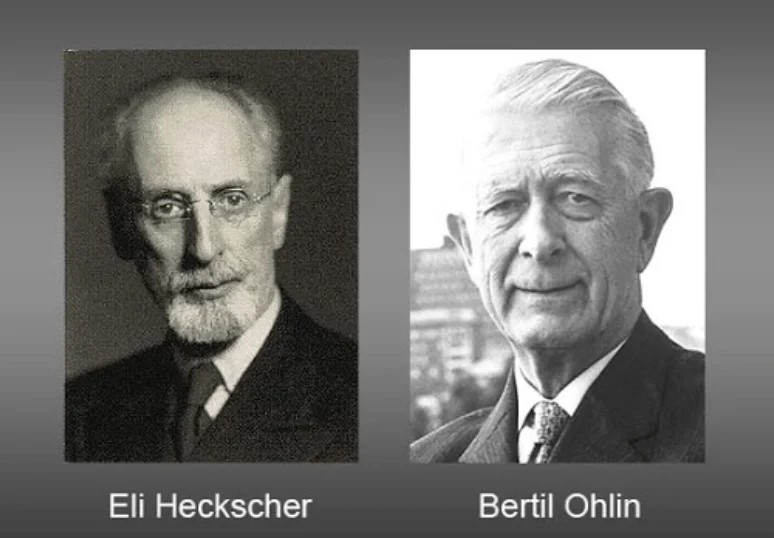
\includegraphics[width=0.5\linewidth]{figs/heckscher-ohlin.jpeg}
\end{figure}

\begin{itemize}
    \item Hecksher: Swedish economist, 1879-1952
    \item Published 1148 books and articles: $\sim$ 16 for every year he was alive!
    \item Ohlin: Swedish economist, 1899-1979
    \item His advisor was Eli Heckscher; won the Nobel Prize in
1977
\end{itemize}

\end{frame}


\begin{frame}{The Heckscher-Ohlin Trade Model}
    \begin{wideitemize}
        \item \blue{Number} of factors of production: 2 (labor $L$, capital $K$)\\
        \qquad \textcolor{gray}{(no specific factors)}
        
    \item<2-> \blue{Mobility} of factors of production:
    \begin{itemize}
        \item Labor is mobile across sectors 
        \item Capital is... also mobile across sectors \\
        \qquad \textcolor{gray}{(question: what is the implication for factor prices?)}
    \end{itemize}

    \item<3-> Number of \blue{sectors} (goods): 2 
    \begin{itemize}
        \item \blue{Tech} output $Y_T$ uses $K$ and $L$
        \item \blue{Cloth} output $Y_C$ also uses $K$ and $L$
        \item But tech is more capital intensive than cloth \\
    \end{itemize}

    \item<4-> Perfect competition; no trade costs

    \item<5-> \blue{Key force}: Differences in factor intensities and endowments
    \end{wideitemize}    
\end{frame}

\section{Production}

\begin{frame}{Production}

    \begin{wideitemize}

        \item<1-> Production of two sectors tech \blue{$T$} and cloth \blue{$C$} in country $i$ use the same factors:
        \begin{eqnarray*}\label{eq: production}
         Y_{i,C} = K_{i,C}^{\beta_C} L_{i,C}^{1-\beta_C}, \qquad  Y_{i,T} = K_{i,T}^{\beta_T} L_{i,T}^{1-\beta_T}
        \end{eqnarray*}

        \item<2-> ... but they have different factor intensities!
        \item<3-> Specifically, we assume $\beta_T > \beta_C$. \blue{What does this mean?}
        \item<4-> Marginal return to capital in $T$ is higher
        \item<5-> For same level of $K,L$, additional $K$ more productive in tech
    \end{wideitemize}
\end{frame}


\begin{frame}{Decreasing marginal returns in capital (holding labor fixed)}

\begin{columns}[T] % align columns
\begin{column}{.5\textwidth}
            \centering
        \begin{tikzpicture}
        
        \pgfmathsetmacro{\beta}{1/4}    % preference for computers
        \pgfmathsetmacro{\K}{1}    % labor endowment
        \pgfmathsetmacro{\A}{1}    % labor endowment
        
        \centering
        \begin{axis}[
            ylabel={$Y_{i,T} = K_{i,T}^{3/4} L_{i,T}^{1/4}$ },
            xlabel={Used input: $K_{i,T}$},
            ymin=0, ymax=3,
            xmin=0, xmax=5,
            yticklabel=\empty,
            xticklabel=\empty,
            axis lines=left,
            enlargelimits=false,
            clip=false,
            axis on top,
            scaled x ticks=false,
            width=7cm, height=7cm,
            title style={font=\bfseries}
        ]
        
        % PPF: Q_C = (L/a_C) - (a_R/a_C) * Q_R
        \addplot[thick, black, domain=0:4] {\A*\K^(\beta)*x^(1-\beta)};
        \addplot+[mark=*,only marks,mark size=1.5pt,black]
                      coordinates { (2, {\A*\K^(\beta)*2^(1-\beta)})};   
        \addplot[dashed, gray] coordinates {(2, 0) (2, {\A*\K^(\beta)*2^(1-\beta)})};
        \node[anchor=north] at (axis cs:2, 0) {\scriptsize $K_{i,T}$};
        \addplot[dashed, gray] coordinates {(0, {\A*\K^(\beta)*2^(1-\beta)}) (2, {\A*\K^(\beta)*2^(1-\beta)})};
        \node[anchor=east] at (axis cs:0, {\A*\K^(\beta)*2^(1-\beta)}) {\scriptsize $Y_{i,T}$};

        \end{axis}
        
        \end{tikzpicture}

                
    \end{column}
    \begin{column}{.5\textwidth}

            \centering
        \begin{tikzpicture}
        
        \pgfmathsetmacro{\beta}{2/3}    % preference for computers
        \pgfmathsetmacro{\K}{1}    % labor endowment
        \pgfmathsetmacro{\A}{1}    % labor endowment
        
        \centering
        \begin{axis}[
            ylabel={$Y_{i,C} =  K_{i,C}^{1/3} L_{i,C}^{2/3}$ },
            xlabel={Used input: $K_{i,C}$},
            ymin=0, ymax=3,
            xmin=0, xmax=5,
            yticklabel=\empty,
            xticklabel=\empty,
            axis lines=left,
            enlargelimits=false,
            clip=false,
            axis on top,
            scaled x ticks=false,
            width=7cm, height=7cm,
            title style={font=\bfseries}
        ]
        
        % PPF: Q_C = (L/a_C) - (a_R/a_C) * Q_R
        \addplot[thick, black, domain=0:4] {\A*\K^(\beta)*x^(1-\beta)};
        \addplot+[mark=*,only marks,mark size=1.5pt,black]
                      coordinates { (2, {\A*\K^(\beta)*2^(1-\beta)})};   
        \addplot[dashed, gray] coordinates {(2, 0) (2, {\A*\K^(\beta)*2^(1-\beta)})};
        \node[anchor=north] at (axis cs:2, 0) {\scriptsize $K_{i,C}$};
        \addplot[dashed, gray] coordinates {(0, {\A*\K^(\beta)*2^(1-\beta)}) (2, {\A*\K^(\beta)*2^(1-\beta)})};
        \node[anchor=east] at (axis cs:0, {\A*\K^(\beta)*2^(1-\beta)}) {\scriptsize $Y_{i,C}$};

        \end{axis}
        
        \end{tikzpicture}
    \end{column}
\end{columns}
\end{frame}


\begin{frame}{Decreasing marginal returns in labor (holding capital fixed)}

\begin{columns}[T] % align columns
\begin{column}{.5\textwidth}
            \centering
        \begin{tikzpicture}
        
        \pgfmathsetmacro{\beta}{3/4}    % preference for computers
        \pgfmathsetmacro{\K}{1}    % labor endowment
        \pgfmathsetmacro{\A}{1}    % labor endowment
        
        \centering
        \begin{axis}[
            ylabel={$Y_{i,T} = K_{i,T}^{3/4} L_{i,T}^{1/4}$ },
            xlabel={Used input: $L_{i,T}$},
            ymin=0, ymax=3,
            xmin=0, xmax=5,
            yticklabel=\empty,
            xticklabel=\empty,
            axis lines=left,
            enlargelimits=false,
            clip=false,
            axis on top,
            scaled x ticks=false,
            width=7cm, height=7cm,
            title style={font=\bfseries}
        ]
        
        % PPF: Q_C = (L/a_C) - (a_R/a_C) * Q_R
        \addplot[thick, black, domain=0:4] {\A*\K^(\beta)*x^(1-\beta)};
        \addplot+[mark=*,only marks,mark size=1.5pt,black]
                      coordinates { (2, {\A*\K^(\beta)*2^(1-\beta)})};   
        \addplot[dashed, gray] coordinates {(2, 0) (2, {\A*\K^(\beta)*2^(1-\beta)})};
        \node[anchor=north] at (axis cs:2, 0) {\scriptsize $L_{i,T}$};
        \addplot[dashed, gray] coordinates {(0, {\A*\K^(\beta)*2^(1-\beta)}) (2, {\A*\K^(\beta)*2^(1-\beta)})};
        \node[anchor=east] at (axis cs:0, {\A*\K^(\beta)*2^(1-\beta)}) {\scriptsize $Y_{i,T}$};

        \end{axis}
        
        \end{tikzpicture}

                
    \end{column}
    \begin{column}{.5\textwidth}

            \centering
        \begin{tikzpicture}
        
        \pgfmathsetmacro{\beta}{1/3}    % preference for computers
        \pgfmathsetmacro{\K}{1}    % labor endowment
        \pgfmathsetmacro{\A}{1}    % labor endowment
        
        \centering
        \begin{axis}[
            ylabel={$Y_{i,C} =  K_{i,C}^{1/3} L_{i,C}^{2/3}$ },
            xlabel={Used labor input: $L_{i,C}$},
            ymin=0, ymax=3,
            xmin=0, xmax=5,
            yticklabel=\empty,
            xticklabel=\empty,
            axis lines=left,
            enlargelimits=false,
            clip=false,
            axis on top,
            scaled x ticks=false,
            width=7cm, height=7cm,
            title style={font=\bfseries}
        ]
        
        % PPF: Q_C = (L/a_C) - (a_R/a_C) * Q_R
        \addplot[thick, black, domain=0:4] {\A*\K^(\beta)*x^(1-\beta)};
        \addplot+[mark=*,only marks,mark size=1.5pt,black]
                      coordinates { (2, {\A*\K^(\beta)*2^(1-\beta)})};   
        \addplot[dashed, gray] coordinates {(2, 0) (2, {\A*\K^(\beta)*2^(1-\beta)})};
        \node[anchor=north] at (axis cs:2, 0) {\scriptsize $L_{i,C}$};
        \addplot[dashed, gray] coordinates {(0, {\A*\K^(\beta)*2^(1-\beta)}) (2, {\A*\K^(\beta)*2^(1-\beta)})};
        \node[anchor=east] at (axis cs:0, {\A*\K^(\beta)*2^(1-\beta)}) {\scriptsize $Y_{i,C}$};

        \end{axis}
        
        \end{tikzpicture}
    \end{column}
\end{columns}
\end{frame}



\begin{frame}{Capital and Labor jointly}

\begin{columns}[T] % align columns
\begin{column}{.8\textwidth}
  \makebox[\linewidth][c]{
    \resizebox{\linewidth}{!}{
    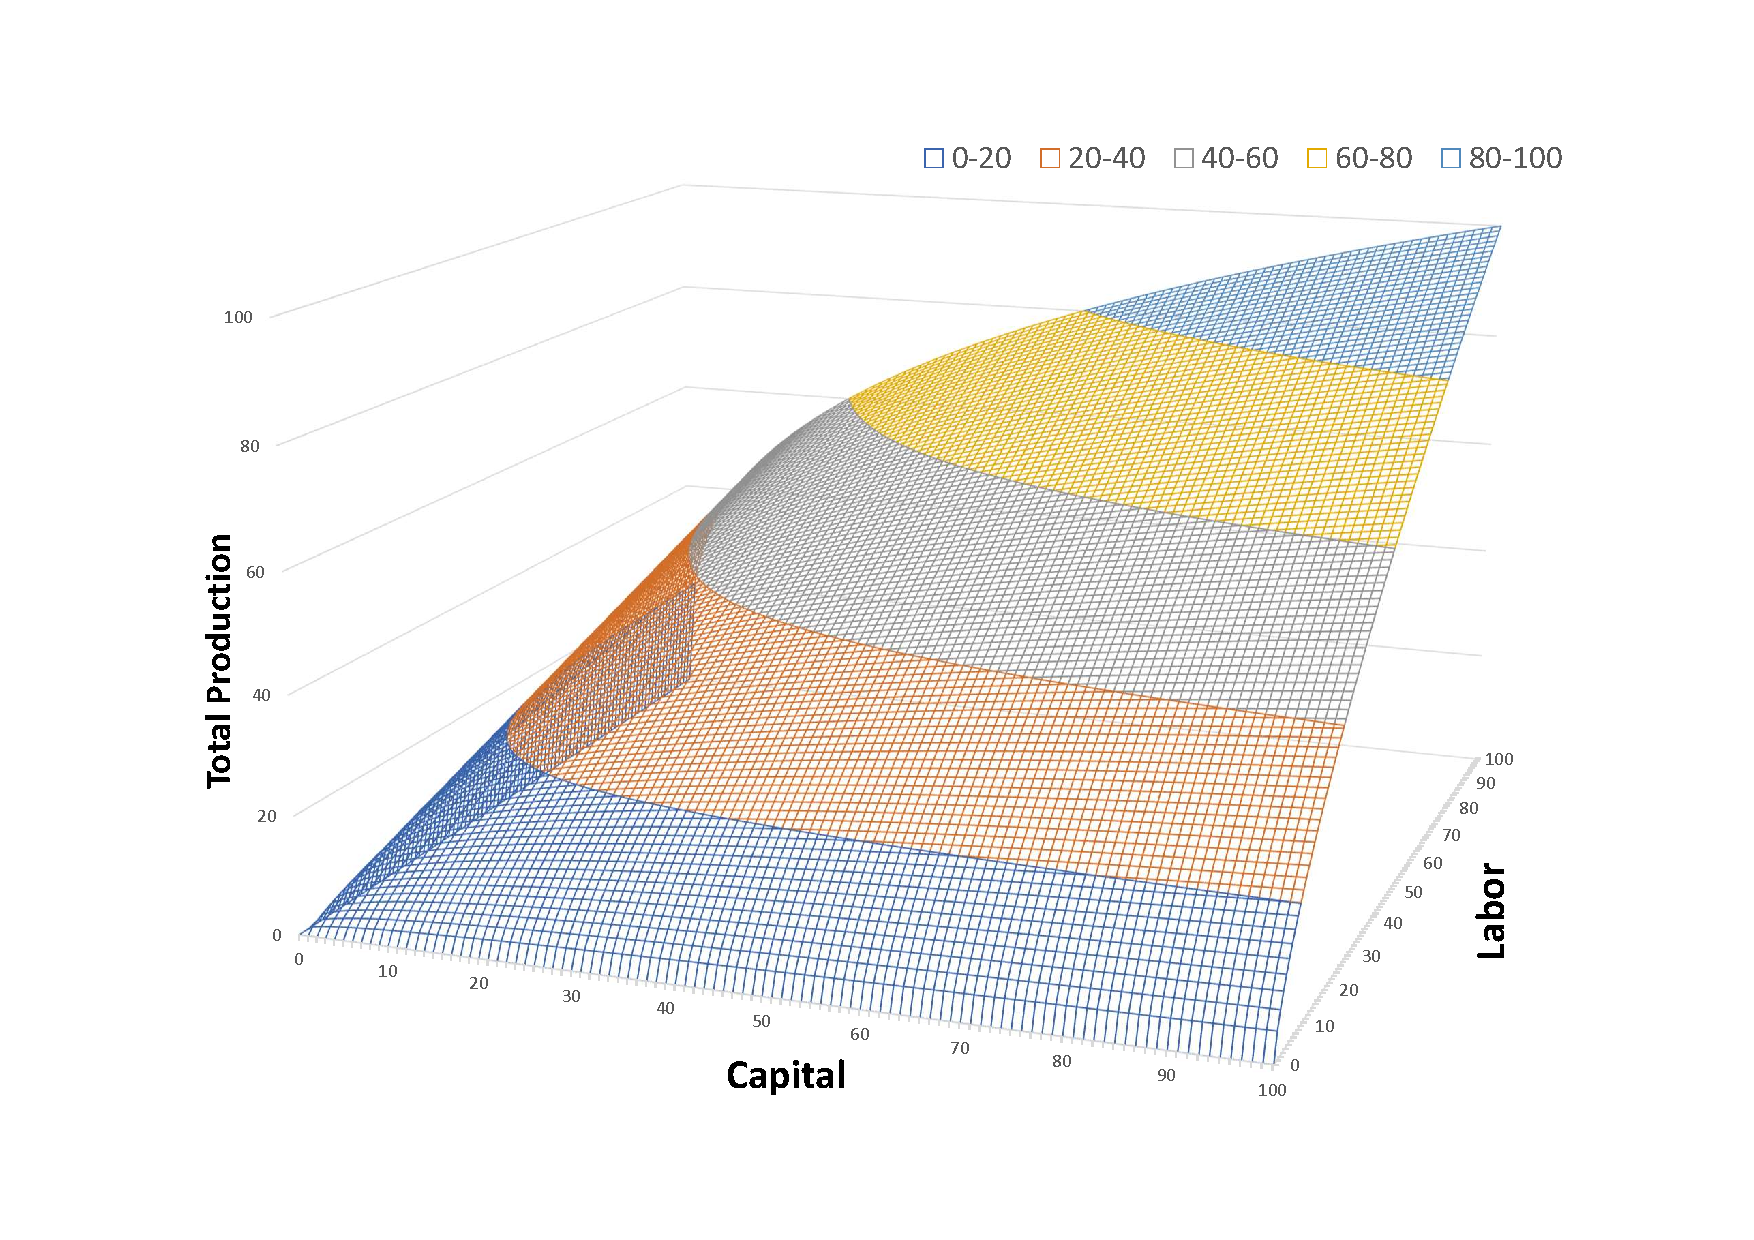
\includegraphics[width=\linewidth]{figs/cobb-douglas-crs.pdf}
      }
    }
\end{column}%
\hfill%
\begin{column}{.2\textwidth}
\begin{eqnarray*}
    Y &=& K^{1/3} L^{2/3} 
\end{eqnarray*}

Cobb-Douglas is Constant Returns to Scale in Capital and Labor jointly... but diminishing marginal returns while holding the other factor fixed...
\end{column}%
\end{columns}

\end{frame}

\begin{frame}{Optimality conditions}
\begin{wideitemize}
    
        \item At their optimal points, factor prices equal their marginal (revenue) product for labor...
        \begin{eqnarray*}
            P_T \times MPL_{i,T} = P_T \times  \frac{\partial Y_{i,T}}{\partial L_{i,T}} &=& w_i\\
            P_C \times MPL_{i,C} = P_C \times  \frac{\partial Y_{i,C}}{\partial L_{i,C}} &=& w_i 
        \end{eqnarray*}

        \item<2-> ... and for capital, respectively:

                \begin{eqnarray*}
            P_T \times MPK_{i,T} =  P_T \times  \frac{\partial Y_{i,T}}{\partial K_{i,T}} &=&r_{i} \\
            P_C \times MPK_{i,C} = P_C \times  \frac{\partial Y_{i,C}}{\partial K_{i,C}} &=& r_{i}
        \end{eqnarray*}

        \item<3-> Note there since factors are mobile, there are common factor prices $\{w_i,r_i\}$. \blue{Why}?

\end{wideitemize}    
\end{frame}

\begin{frame}{Factor mobility}
\begin{wideitemize}
    
        \item \blue{Claim}: since factors are mobile, then there are common factor prices $\{w_i,r_i\}$.

        \item<2-> Proof by contradiction (sketch):
        \begin{itemize}
            \item<3-> Suppose that wages in one sector are larger than the other $w_{i,g} > w_{i,g'}$
            \item<4-> $\implies$ It would be optimal for workers to switch from the low to high paying sector
            \item<5-> $\implies$ Production would only happen in one sector, but both sectors are demanded in eqm
            \item<6-> $\implies$ Contradiction
            \item<7-> Initial supposition is wrong $\implies$ wages must be equal in eqm 
        \end{itemize}

        \item<8->  Same reasoning is valid for $r_i$

\end{wideitemize}    
\end{frame}

\begin{frame}{Factor mobility}
\begin{wideitemize}
    
        \item Wage rage \blue{$w_i$} will be such that
        \begin{eqnarray*}
            & & L_{i,C} + L_{i,T} = \bar{L}_i  \qquad \text{and} \\
            & & P_T \times MPL_{i,T} = w_i = 
            P_C \times MPL_{i,C} \\
            & & \textcolor{gray}{P_{C} \times (1-\beta_C) \times \left( \frac{K_{i,C}}{L_{i,C}} \right)^{\beta_C} = w_i = P_{T} \times (1-\beta_T) \times \left( \frac{K_{i,T}}{L_{i,T}} \right)^{\beta_T}}
        \end{eqnarray*}

        \item<2-> Rental rage \blue{$r_i$} will be such that
        \begin{eqnarray*}
            & & K_{i,C} + K_{i,T} = \bar{L}_i \qquad \text{and} \\
            & & P_T \times MPK_{i,T} = r_i = 
            P_C \times MPK_{i,C}   \\
            & & \textcolor{gray}{P_{C} \times  \beta_C \times \left( \frac{L_{i,C}}{K_{i,C}} \right)^{1-\beta_C} = r_i = P_{T}  \times \beta_T \times \left( \frac{L_{i,T}}{K_{i,T}} \right)^{1-\beta_T}}
        \end{eqnarray*}


\end{wideitemize}    
\end{frame}

\begin{frame}{Factor intensities}
\begin{wideitemize}
    
        \item Cloth production is relatively labor-intensive
        \item Tech production is relatively capital-intensive

        \item<2-> With two sectors and two factors of production, the tech sector is relatively capital-intensive if, at any wage-rental ratio $w_i/r_i$,

        \begin{eqnarray*}
            \frac{K_{i,T}}{L_{i,T}} > \frac{K_{i,C}}{L_{i,C}} 
        \end{eqnarray*}

\end{wideitemize}    
\end{frame}


\begin{frame}{From factor prices to optimal choices}

        \begin{wideitemize}
            \item Recall:
            \begin{eqnarray*}
                P_T \times MPL_{i,T} = P_T \times  \frac{\partial Y_{i,T}}{\partial L_{i,T}} = w_i, \qquad P_T \times MPK_{i,T} =  P_T \times  \frac{\partial Y_{i,T}}{\partial K_{i,T}} &=&r_{i}
            \end{eqnarray*}

            \item<2-> Combining these:
                \begin{eqnarray*}
                \frac{P_{T} \times (1-\beta_T) \times \left( \frac{K_{i,T}}{L_{i,T}} \right)^{\beta_T}}{P_{T}  \times \beta_T \times \left( \frac{L_{i,T}}{K_{i,T}} \right)^{1-\beta_T}} &=& \frac{w_i}{r_i} \iff \frac{K_{i,T}}{L_{i,T}} = \frac{\beta_T}{1-\beta_T} \times \frac{w_i}{r_i} 
                \end{eqnarray*}

                \item<3-> Same valid for $C$. So both sectors' capital-to-labor ratios pinned down by relative factor prices:
\begin{eqnarray*}\label{eq: capital-labor}
    \frac{K_{i,C}}{L_{i,C}} = \frac{\beta_C}{1-\beta_C} \times \frac{w_i}{r_i}, \qquad \frac{K_{i,T}}{L_{i,T}} = \frac{\beta_T}{1-\beta_T} \times \frac{w_i}{r_i} 
\end{eqnarray*}        

    \item<4-> Since $\beta_T > \beta_C$, for any prices $\frac{w_i}{r_i}$, it will be the case that $\frac{K_{i,T}}{L_{i,T}} > \frac{K_{i,C}}{L_{i,C}} $.

\end{wideitemize}
\end{frame}


\begin{frame}{Graphical representation}

\begin{columns}[T] % align columns
\begin{column}{.5\textwidth}
            \centering
    \begin{tikzpicture}
    \begin{axis}[
        axis lines=middle,
        xmin=0, xmax=1.1,
        ymin=0, ymax=1.1,
    %    xlabel={\small Output of manufactures / Labor in manufactures},
    %    ylabel={\small Output of food / Labor in food},
        xtick=\empty,
        ytick=\empty,
        width=8cm,
        height=8cm,
        axis line style={->},
        clip=false,
        enlargelimits=false,
        domain=0.0:1,
        samples=200
    ]
    

    \node[anchor=west] at (axis cs:1.1,0) {  $K_{i,g}/L_{i,g}$};
    \node[anchor=south] at (axis cs:0,1.1) { $w_i/r_i$};
    
    \end{axis}
    
    \end{tikzpicture}

                
    \end{column}
    \begin{column}{.5\textwidth}

    \begin{wideitemize}
        \item Let's place $K_{i,g}/L_{i,g}$ on the x-ais and $w_i/r_i$ on the y-axis
    \end{wideitemize}


    \end{column}
\end{columns}
\end{frame}


\begin{frame}{Graphical representation}
\addtocounter{framenumber}{-1}

\begin{columns}[T] % align columns
\begin{column}{.5\textwidth}
            \centering
    \begin{tikzpicture}
    \begin{axis}[
        axis lines=middle,
        xmin=0, xmax=1.1,
        ymin=0, ymax=1.1,
    %    xlabel={\small Output of manufactures / Labor in manufactures},
    %    ylabel={\small Output of food / Labor in food},
        xtick=\empty,
        ytick=\empty,
        width=8cm,
        height=8cm,
        axis line style={->},
        clip=false,
        enlargelimits=false,
        domain=0.0:1,
        samples=200
    ]
    
    \pgfmathsetmacro{\a}{0.5}       % curvature parameter
    \pgfmathsetmacro{\betac}{1/3}       % curvature parameter
    \pgfmathsetmacro{\betat}{2/3}       % curvature parameter
    \pgfmathsetmacro{\c}{(\betac)^(\betac)*(1-\betac)^(1-\betac)}        \pgfmathsetmacro{\t}{(\betat)^(\betat)*(1-\betat)^(1-\betat)}        \pgfmathsetmacro{\rw}{1/4}
    \pgfmathsetmacro{\prw}{-(\c / \t * (\rw)^(\betat- \betac)}
    \pgfmathsetmacro{\rww}{1/2}
    \pgfmathsetmacro{\prww}{-(\c / \t * (\rww)^(\betat- \betac)}
    % curvature parameter
% curvature parameter
    
    \addplot[brown] ({x}, {(1-\betat)/\betat * x});
    \addplot[red, domain=0:0.5] ({x}, {(1-\betac)/\betac * x});
    \node[anchor=west] at (axis cs:1.1,0) {  $K_{i,g}/L_{i,g}$};
    \node[anchor=south] at (axis cs:0,1.1) { $w_i/r_i$};

    % slope
    \pgfmathsetmacro{\rws}{3/4}
    \addplot[dashed, gray] coordinates {(\betac / (1-\betac) * \rws, \rws) (\betac / (1-\betac) * (\rws + .2), \rws) };
    \node[anchor=north west] at (axis cs:{\betac / (1-\betac) * \rws}, \rws) {$1$};
    \addplot[dashed, gray] coordinates {(\betac / (1-\betac) * (\rws + .2), \rws) (\betac / (1-\betac) * (\rws + .2), \rws + .2)  };
    \node[anchor=south west] at (axis cs:{\betac / (1-\betac) * (\rws + .2)}, \rws) {$\frac{1-\beta_C}{\beta_C}$};

    \pgfmathsetmacro{\rwss}{0.3}
    \addplot[dashed, gray] coordinates {(\betat / (1-\betat) * \rwss, \rwss) (\betat / (1-\betat) * (\rwss + .065), \rwss) };
    \node[anchor=north west] at (axis cs:{\betat / (1-\betat) * \rwss}, \rwss) {$1$};
    \addplot[dashed, gray] coordinates {(\betat / (1-\betat) * (\rwss + .065), \rwss) (\betat / (1-\betat) * (\rwss + .065), \rwss + .065)  };
    \node[anchor=south west] at (axis cs:{\betat / (1-\betat) * (\rwss + .065)}, \rwss-.05) {$\frac{1-\beta_T}{\beta_T}$};
     \end{axis}
    
    \end{tikzpicture}

                
    \end{column}
    \begin{column}{.5\textwidth}

    \begin{wideitemize}
        \item Let's place $K_{i,g}/L_{i,g}$ on the x-ais and $w_i/r_i$ on the y-axis

    \item Inverting equations, $\frac{w_i}{r_i} = \frac{1-\beta_g}{\beta_g} \times \frac{K_{i,g}}{L_{i,g}}$

    \item Curve for $C$ steeper than for $T$
    \end{wideitemize}


    \end{column}
\end{columns}
\end{frame}

\begin{frame}{Graphical representation}
\addtocounter{framenumber}{-1}

\begin{columns}[T] % align columns
\begin{column}{.5\textwidth}
            \centering
    \begin{tikzpicture}
    \begin{axis}[
        axis lines=middle,
        xmin=0, xmax=1.1,
        ymin=0, ymax=1.1,
    %    xlabel={\small Output of manufactures / Labor in manufactures},
    %    ylabel={\small Output of food / Labor in food},
        xtick=\empty,
        ytick=\empty,
        width=8cm,
        height=8cm,
        axis line style={->},
        clip=false,
        enlargelimits=false,
        domain=0.0:1,
        samples=200
    ]
    
    \pgfmathsetmacro{\a}{0.5}       % curvature parameter
    \pgfmathsetmacro{\betac}{1/3}       % curvature parameter
    \pgfmathsetmacro{\betat}{2/3}       % curvature parameter
    \pgfmathsetmacro{\c}{(\betac)^(\betac)*(1-\betac)^(1-\betac)}        \pgfmathsetmacro{\t}{(\betat)^(\betat)*(1-\betat)^(1-\betat)}        \pgfmathsetmacro{\rw}{1/4}
    \pgfmathsetmacro{\prw}{-(\c / \t * (\rw)^(\betat- \betac)}
    \pgfmathsetmacro{\rww}{1/2}
    \pgfmathsetmacro{\prww}{-(\c / \t * (\rww)^(\betat- \betac)}
    % curvature parameter
% curvature parameter
    
    \addplot[brown] ({x}, {(1-\betat)/\betat * x});
    \addplot[red, domain=0:0.5] ({x}, {(1-\betac)/\betac * x});
    \node[anchor=west] at (axis cs:1.1,0) {  $K_{i,g}/L_{i,g}$};
    \node[anchor=south] at (axis cs:0,1.1) { $w_i/r_i$};

    %old eqm
    \addplot[dashed, gray] coordinates {(0, \rw) (\betat / (1-\betat) * \rw, \rw)};
    \addplot[mark=*, black, mark size=1.5pt] coordinates {(0,\rw)};
    \node[anchor=south east] at (axis cs:0,\rw) {$\frac{w_i}{r_i}$};
    \addplot[mark=*, black, mark size=1.5pt] coordinates {(\betac / (1-\betac) * \rw,\rw)};
    \addplot[dashed, gray] coordinates {(\betac / (1-\betac) * \rw, \rw) (\betac / (1-\betac) * \rw , 0)};
    \node[anchor=north] at (axis cs:{\betac / (1-\betac) * \rw} , 0) {$\frac{K_C}{L_C}$};
    \addplot[mark=*, black, mark size=1.5pt] coordinates {(\betat / (1-\betat) * \rw,\rw)};
    \addplot[dashed, gray] coordinates {(\betat / (1-\betat) * \rw, \rw) (\betat / (1-\betat) * \rw , 0)};
    \node[anchor=north] at (axis cs:{\betat / (1-\betat) * \rw} , 0) {$\frac{K_T}{L_T}$};

    %new eqm
    \addplot[dashed, gray] coordinates {(0, \rww) (\betat / (1-\betat) * \rww, \rww)};
    \addplot[mark=*, black, mark size=1.5pt] coordinates {(0,\rww)};
    \node[anchor=south east] at (axis cs:0,\rww) {$\left( \frac{w_i}{r_i} \right)'$};
    \addplot[mark=*, black, mark size=1.5pt] coordinates {(\betac / (1-\betac) * \rww,\rww)};
    \addplot[dashed, gray] coordinates {(\betac / (1-\betac) * \rww, \rww) (\betac / (1-\betac) * \rww , 0)};
    \node[anchor=north] at (axis cs:{\betac / (1-\betac) * \rww} , 0) {$\frac{K_C'}{L_C'}$};
    \addplot[mark=*, black, mark size=1.5pt] coordinates {(\betat / (1-\betat) * \rww,\rww)};
    \addplot[dashed, gray] coordinates {(\betat / (1-\betat) * \rww, \rww) (\betat / (1-\betat) * \rww , 0) };
    \node[anchor=north] at (axis cs:{\betat / (1-\betat) * \rww} , 0) {$\frac{K_T'}{L_T'}$};

    % slope
    \pgfmathsetmacro{\rws}{3/4}
    \addplot[dashed, gray] coordinates {(\betac / (1-\betac) * \rws, \rws) (\betac / (1-\betac) * (\rws + .2), \rws) };
    \node[anchor=north west] at (axis cs:{\betac / (1-\betac) * \rws}, \rws) {$1$};
    \addplot[dashed, gray] coordinates {(\betac / (1-\betac) * (\rws + .2), \rws) (\betac / (1-\betac) * (\rws + .2), \rws + .2)  };
    \node[anchor=south west] at (axis cs:{\betac / (1-\betac) * (\rws + .2)}, \rws) {$\frac{1-\beta_C}{\beta_C}$};

    \pgfmathsetmacro{\rwss}{0.3}
    \addplot[dashed, gray] coordinates {(\betat / (1-\betat) * \rwss, \rwss) (\betat / (1-\betat) * (\rwss + .065), \rwss) };
    \node[anchor=north west] at (axis cs:{\betat / (1-\betat) * \rwss}, \rwss) {$1$};
    \addplot[dashed, gray] coordinates {(\betat / (1-\betat) * (\rwss + .065), \rwss) (\betat / (1-\betat) * (\rwss + .065), \rwss + .065)  };
    \node[anchor=south west] at (axis cs:{\betat / (1-\betat) * (\rwss + .065)}, \rwss-.05) {$\frac{1-\beta_T}{\beta_T}$};
     \end{axis}
    
    \end{tikzpicture}

                
    \end{column}
    \begin{column}{.5\textwidth}

    \begin{wideitemize}
        \item Let's place $K_{i,g}/L_{i,g}$ on the x-ais and $w_i/r_i$ on the y-axis

        \item Let's place $K_{i,g}/L_{i,g}$ on the x-ais and $w_i/r_i$ on the y-axis

    \item Inverting equations, $\frac{w_i}{r_i} = \frac{1-\beta_g}{\beta_g} \times \frac{K_{i,g}}{L_{i,g}}$

    \item Curve for $C$ steeper than for $T$

    \item Relative factor prices pin down capital to labor ratio
    \end{wideitemize}
    


    \end{column}
\end{columns}
\end{frame}

\begin{frame}{From goods prices to optimal choices}

        \begin{wideitemize}
            \item Recall:
                \begin{eqnarray*}
            P_T \times MPK_{i,T} =  P_T \times  \frac{\partial Y_{i,T}}{\partial K_{i,T}} = r_{i}, \qquad P_C \times MPK_{i,C} = P_C \times  \frac{\partial Y_{i,C}}{\partial K_{i,C}} = r_{i}
        \end{eqnarray*}

            \item<2-> Combining these:
\begin{eqnarray*}
    \frac{P_C}{P_T} = \frac{MPL_{i,T}}{MPL_{i,C}} \iff 
    \frac{P_C}{P_T} = \frac{(1-\beta_T) \times \left( \frac{K_{i,T}}{L_{i,T}} \right)^{\beta_T}}{ (1-\beta_C) \times \left( \frac{K_{i,C}}{L_{i,C}} \right)^{\beta_C}}  
\end{eqnarray*}

                \item<3-> But we have just shown $K/L$ is a function of $w/r$. Hence:
                
\begin{eqnarray*}\label{eq: goods-factor-prices}
    \frac{P_C}{P_T} = \frac{(1-\beta_T) \times \left( \frac{\beta_T}{1-\beta_T} \times \frac{w_i}{r_i}  \right)^{\beta_T}}{ (1-\beta_C) \times \left( \frac{\beta_C}{1-\beta_C} \times \frac{w_i}{r_i} \right)^{\beta_C}} \iff \frac{P_C}{P_T} = \frac{(1-\beta_T)^{1-\beta_T} \beta_T^{\beta_T}}{ (1-\beta_C)^{1-\beta_C} \beta_C^{\beta_C} } \times \left(  \frac{w_i}{r_i} \right)^{\beta_T - \beta_C}
\end{eqnarray*} 


\end{wideitemize}
\end{frame}

\section{Stolper-Samuelson Theorem}

\begin{frame}{Stolper-Samuelson Theorem}

        \begin{wideitemize}
            \item \blue{Statement}:

            \begin{quote}
                If the relative price of one good increases, the \textbf{real income} of the factor that is used intensively in production of the good will increase, while the other factor’s real income falls.
            \end{quote}

            \item<2-> \blue{Magnification effect}:

            \begin{equation*}
            \hat{w}_i > \hat{P}_C > \hat{P}_T > \hat{r}_i 
         \end{equation*}

         \textcolor{gray}{(where $\hat{x} = (x'-x)/x$ is the percent change in variable $x$)}

         \item<3-> Using our specific function form:
    \begin{eqnarray*}\label{eq: goods-factor-prices}
         \frac{P_C}{P_T} = \text{constant} \times \left(  \frac{w_i}{r_i} \right)^{\beta_T - \beta_C}, \qquad \text{with } 0<\beta_C<\beta_T<1
    \end{eqnarray*}         
    
\end{wideitemize}
\end{frame}


\begin{frame}{Graphical representation}

\begin{columns}[T] % align columns
\begin{column}{.5\textwidth}
            \centering
    \begin{tikzpicture}
    \begin{axis}[
        axis lines=middle,
        xmin=0, xmax=1.1,
        ymin=0, ymax=1.1,
    %    xlabel={\small Output of manufactures / Labor in manufactures},
    %    ylabel={\small Output of food / Labor in food},
        xtick=\empty,
        ytick=\empty,
        width=8cm,
        height=8cm,
        axis line style={->},
        clip=false,
        enlargelimits=false,
        domain=0.0:1,
        samples=200
    ]
    
    \pgfmathsetmacro{\a}{0.5}       % curvature parameter
    \pgfmathsetmacro{\betac}{1/3}       % curvature parameter
    \pgfmathsetmacro{\betat}{2/3}       % curvature parameter
    \pgfmathsetmacro{\c}{(\betac)^(\betac)*(1-\betac)^(1-\betac)}        \pgfmathsetmacro{\t}{(\betat)^(\betat)*(1-\betat)^(1-\betat)}        \pgfmathsetmacro{\rw}{1/4}
    \pgfmathsetmacro{\prw}{-(\c / \t * (\rw)^(\betat- \betac)}
    \pgfmathsetmacro{\rww}{1/2}
    \pgfmathsetmacro{\prww}{-(\c / \t * (\rww)^(\betat- \betac)}
    % curvature parameter
% curvature parameter
    
    \addplot[blue] ({x}, {\t / \c * (x)^(1/(\betat - \betac))});
    \node[anchor=west] at (axis cs:1.1,0) {  $P_C / P_T$};
    \node[anchor=south] at (axis cs:0,1.1) { $w_i/r_i$};


 \end{axis}
    
    \end{tikzpicture}

                
    \end{column}
    \begin{column}{.5\textwidth}

    \begin{wideitemize}
        \item Let's place $P_C/P_T$ on the x-ais and $w_i/r_i$ on the y-axis

    \item Inverting equation, $\frac{w_i}{r_i} = \left( \frac{1}{\text{constant}} \times  \frac{P_{C}}{P_{T}} \right)^{\frac{1}{\beta_T-\beta_C}}$

    \item \blue{Convex} function:  $w_i/r_i$ grows more than proportionately in $P_C / P_T$
    
    \end{wideitemize}


    \end{column}
\end{columns}
\end{frame}

\begin{frame}{Putting everything together...}

        \begin{wideitemize}
            \item We first mapped $w_i/r_i \mapsto K_{i,g}/L_{i,g}$:
\begin{eqnarray*}\label{eq: capital-labor}
    \frac{K_{i,C}}{L_{i,C}} = \frac{\beta_C}{1-\beta_C} \times \frac{w_i}{r_i}, \qquad \frac{K_{i,T}}{L_{i,T}} = \frac{\beta_T}{1-\beta_T} \times \frac{w_i}{r_i} 
\end{eqnarray*}        
            \item We then mapped $P_C/P_T \mapsto w_i/r_i$:

            \begin{equation*}
                \frac{w_i}{r_i} = \left( \frac{1}{\text{constant}} \times  \frac{P_{C}}{P_{T}} \right)^{\frac{1}{\beta_T-\beta_C}}
            \end{equation*}

            \item Putting these together, we can pin down from relative prices $P_C / P_T \mapsto K_{i,g}/L_{i,g}$:

            \begin{equation*}
                \frac{K_{i,g}}{L_{i,g}} = \text{constant}_g \times  \left(  \frac{P_{C}}{P_{T}} \right)^{\frac{1}{\beta_T-\beta_C}}
            \end{equation*}

\end{wideitemize}
\end{frame}


\begin{frame}{Signature chart}
    \centering
    \begin{tikzpicture}
    \begin{axis}[
        axis lines=middle,
        xmin=-1.1, xmax=1.1,
        ymin=0, ymax=1.1,
    %    xlabel={\small Output of manufactures / Labor in manufactures},
    %    ylabel={\small Output of food / Labor in food},
        xtick=\empty,
        ytick=\empty,
        width=13cm,
        height=8cm,
        axis line style={<->},
        clip=false,
        enlargelimits=false,
        domain=0.0:1,
        samples=200
    ]
    
    \pgfmathsetmacro{\a}{0.5}       % curvature parameter
    \pgfmathsetmacro{\betac}{1/3}       % curvature parameter
    \pgfmathsetmacro{\betat}{2/3}       % curvature parameter
    \pgfmathsetmacro{\c}{(\betac)^(\betac)*(1-\betac)^(1-\betac)}        \pgfmathsetmacro{\t}{(\betat)^(\betat)*(1-\betat)^(1-\betat)}        \pgfmathsetmacro{\rw}{1/4}
    \pgfmathsetmacro{\prw}{-(\c / \t * (\rw)^(\betat- \betac)}
    \pgfmathsetmacro{\rww}{1/2}
    \pgfmathsetmacro{\prww}{-(\c / \t * (\rww)^(\betat- \betac)}
    % curvature parameter
% curvature parameter
    
    % NW: Production function for food (plot in 2nd quadrant)
    \node[anchor=east] at (axis cs:-1.1,0) {  $P_C/P_T$};
    \node[anchor=west] at (axis cs:1.1,0) {  $K_{i,g}/L_{i,g}$};
    \node[anchor=south] at (axis cs:0,1.1) { $w_i/r_i$};


     \end{axis}
    
    \end{tikzpicture}

\end{frame}


\begin{frame}{Signature chart}
\addtocounter{framenumber}{-1}
    \centering
    \begin{tikzpicture}
    \begin{axis}[
        axis lines=middle,
        xmin=-1.1, xmax=1.1,
        ymin=0, ymax=1.1,
    %    xlabel={\small Output of manufactures / Labor in manufactures},
    %    ylabel={\small Output of food / Labor in food},
        xtick=\empty,
        ytick=\empty,
        width=13cm,
        height=8cm,
        axis line style={<->},
        clip=false,
        enlargelimits=false,
        domain=0.0:1,
        samples=200
    ]
    
    \pgfmathsetmacro{\a}{0.5}       % curvature parameter
    \pgfmathsetmacro{\betac}{1/3}       % curvature parameter
    \pgfmathsetmacro{\betat}{2/3}       % curvature parameter
    \pgfmathsetmacro{\c}{(\betac)^(\betac)*(1-\betac)^(1-\betac)}        \pgfmathsetmacro{\t}{(\betat)^(\betat)*(1-\betat)^(1-\betat)}        \pgfmathsetmacro{\rw}{1/4}
    \pgfmathsetmacro{\prw}{-(\c / \t * (\rw)^(\betat- \betac)}
    \pgfmathsetmacro{\rww}{1/2}
    \pgfmathsetmacro{\prww}{-(\c / \t * (\rww)^(\betat- \betac)}
    % curvature parameter
% curvature parameter
    
    % NW: Production function for food (plot in 2nd quadrant)
    \addplot[brown] ({x}, {(1-\betat)/\betat * x});
    \addplot[red, domain=0:0.5] ({x}, {(1-\betac)/\betac * x});
    \node[anchor=east] at (axis cs:-1.1,0) {  $P_C/P_T$};
    \node[anchor=west] at (axis cs:1.1,0) {  $K_{i,g}/L_{i,g}$};
    \node[anchor=south] at (axis cs:0,1.1) { $w_i/r_i$};



    % slope
    \pgfmathsetmacro{\rws}{3/4}
    \addplot[dashed, gray] coordinates {(\betac / (1-\betac) * \rws, \rws) (\betac / (1-\betac) * (\rws + .2), \rws) };
    \node[anchor=north west] at (axis cs:{\betac / (1-\betac) * \rws}, \rws) {$1$};
    \addplot[dashed, gray] coordinates {(\betac / (1-\betac) * (\rws + .2), \rws) (\betac / (1-\betac) * (\rws + .2), \rws + .2)  };
    \node[anchor=south west] at (axis cs:{\betac / (1-\betac) * (\rws + .2)}, \rws) {$\frac{1-\beta_C}{\beta_C}$};

    \pgfmathsetmacro{\rwss}{0.3}
    \addplot[dashed, gray] coordinates {(\betat / (1-\betat) * \rwss, \rwss) (\betat / (1-\betat) * (\rwss + .065), \rwss) };
    \node[anchor=north west] at (axis cs:{\betat / (1-\betat) * \rwss}, \rwss) {$1$};
    \addplot[dashed, gray] coordinates {(\betat / (1-\betat) * (\rwss + .065), \rwss) (\betat / (1-\betat) * (\rwss + .065), \rwss + .065)  };
    \node[anchor=south west] at (axis cs:{\betat / (1-\betat) * (\rwss + .065)}, \rwss-.05) {$\frac{1-\beta_T}{\beta_T}$};
     \end{axis}
    
    \end{tikzpicture}

\end{frame}


\begin{frame}{Signature chart}
\addtocounter{framenumber}{-1}
    \centering
    \begin{tikzpicture}
    \begin{axis}[
        axis lines=middle,
        xmin=-1.1, xmax=1.1,
        ymin=0, ymax=1.1,
    %    xlabel={\small Output of manufactures / Labor in manufactures},
    %    ylabel={\small Output of food / Labor in food},
        xtick=\empty,
        ytick=\empty,
        width=13cm,
        height=8cm,
        axis line style={<->},
        clip=false,
        enlargelimits=false,
        domain=0.0:1,
        samples=200
    ]
    
    \pgfmathsetmacro{\a}{0.5}       % curvature parameter
    \pgfmathsetmacro{\betac}{1/3}       % curvature parameter
    \pgfmathsetmacro{\betat}{2/3}       % curvature parameter
    \pgfmathsetmacro{\c}{(\betac)^(\betac)*(1-\betac)^(1-\betac)}        \pgfmathsetmacro{\t}{(\betat)^(\betat)*(1-\betat)^(1-\betat)}        \pgfmathsetmacro{\rw}{1/4}
    \pgfmathsetmacro{\prw}{-(\c / \t * (\rw)^(\betat- \betac)}
    \pgfmathsetmacro{\rww}{1/2}
    \pgfmathsetmacro{\prww}{-(\c / \t * (\rww)^(\betat- \betac)}
    % curvature parameter
% curvature parameter
    
    % NW: Production function for food (plot in 2nd quadrant)
    \addplot[brown] ({x}, {(1-\betat)/\betat * x});
    \addplot[red, domain=0:0.5] ({x}, {(1-\betac)/\betac * x});
    \addplot[blue] ({-x}, {\t / \c * (x)^(1/(\betat - \betac))});
    \node[anchor=east] at (axis cs:-1.1,0) {  $P_C/P_T$};
    \node[anchor=west] at (axis cs:1.1,0) {  $K_{i,g}/L_{i,g}$};
    \node[anchor=south] at (axis cs:0,1.1) { $w_i/r_i$};



    % slope
    \pgfmathsetmacro{\rws}{3/4}
    \addplot[dashed, gray] coordinates {(\betac / (1-\betac) * \rws, \rws) (\betac / (1-\betac) * (\rws + .2), \rws) };
    \node[anchor=north west] at (axis cs:{\betac / (1-\betac) * \rws}, \rws) {$1$};
    \addplot[dashed, gray] coordinates {(\betac / (1-\betac) * (\rws + .2), \rws) (\betac / (1-\betac) * (\rws + .2), \rws + .2)  };
    \node[anchor=south west] at (axis cs:{\betac / (1-\betac) * (\rws + .2)}, \rws) {$\frac{1-\beta_C}{\beta_C}$};

    \pgfmathsetmacro{\rwss}{0.3}
    \addplot[dashed, gray] coordinates {(\betat / (1-\betat) * \rwss, \rwss) (\betat / (1-\betat) * (\rwss + .065), \rwss) };
    \node[anchor=north west] at (axis cs:{\betat / (1-\betat) * \rwss}, \rwss) {$1$};
    \addplot[dashed, gray] coordinates {(\betat / (1-\betat) * (\rwss + .065), \rwss) (\betat / (1-\betat) * (\rwss + .065), \rwss + .065)  };
    \node[anchor=south west] at (axis cs:{\betat / (1-\betat) * (\rwss + .065)}, \rwss-.05) {$\frac{1-\beta_T}{\beta_T}$};
     \end{axis}
    
    \end{tikzpicture}

\end{frame}


\begin{frame}{Signature chart}
\addtocounter{framenumber}{-1}
    \centering
    \begin{tikzpicture}
    \begin{axis}[
        axis lines=middle,
        xmin=-1.1, xmax=1.1,
        ymin=0, ymax=1.1,
    %    xlabel={\small Output of manufactures / Labor in manufactures},
    %    ylabel={\small Output of food / Labor in food},
        xtick=\empty,
        ytick=\empty,
        width=13cm,
        height=8cm,
        axis line style={<->},
        clip=false,
        enlargelimits=false,
        domain=0.0:1,
        samples=200
    ]
    
    \pgfmathsetmacro{\a}{0.5}       % curvature parameter
    \pgfmathsetmacro{\betac}{1/3}       % curvature parameter
    \pgfmathsetmacro{\betat}{2/3}       % curvature parameter
    \pgfmathsetmacro{\c}{(\betac)^(\betac)*(1-\betac)^(1-\betac)}        \pgfmathsetmacro{\t}{(\betat)^(\betat)*(1-\betat)^(1-\betat)}        \pgfmathsetmacro{\rw}{1/4}
    \pgfmathsetmacro{\prw}{-(\c / \t * (\rw)^(\betat- \betac)}
    \pgfmathsetmacro{\rww}{1/2}
    \pgfmathsetmacro{\prww}{-(\c / \t * (\rww)^(\betat- \betac)}
    % curvature parameter
% curvature parameter
    
    % NW: Production function for food (plot in 2nd quadrant)
    \addplot[brown] ({x}, {(1-\betat)/\betat * x});
    \addplot[red, domain=0:0.5] ({x}, {(1-\betac)/\betac * x});
    \addplot[blue] ({-x}, {\t / \c * (x)^(1/(\betat - \betac))});
    \node[anchor=east] at (axis cs:-1.1,0) {  $P_C/P_T$};
    \node[anchor=west] at (axis cs:1.1,0) {  $K_{i,g}/L_{i,g}$};
    \node[anchor=south] at (axis cs:0,1.1) { $w_i/r_i$};

    %old eqm
    \addplot[dashed, gray] coordinates {(\prw, \rw) (\betat / (1-\betat) * \rw, \rw)};
    \addplot[dashed, gray] coordinates {(\prw, \rw) (\prw , 0)};
    \node[anchor=north] at (axis cs:\prw , 0) {$\frac{P_C}{P_T}$};
    \addplot[mark=*, black, mark size=1.5pt] coordinates {(\prw,\rw)};
    \addplot[mark=*, black, mark size=1.5pt] coordinates {(0,\rw)};
    \node[anchor=south east] at (axis cs:0,\rw) {$\frac{w_i}{r_i}$};
    \addplot[mark=*, black, mark size=1.5pt] coordinates {(\betac / (1-\betac) * \rw,\rw)};
    \addplot[dashed, gray] coordinates {(\betac / (1-\betac) * \rw, \rw) (\betac / (1-\betac) * \rw , 0)};
    \node[anchor=north] at (axis cs:{\betac / (1-\betac) * \rw} , 0) {$\frac{K_C}{L_C}$};
    \addplot[mark=*, black, mark size=1.5pt] coordinates {(\betat / (1-\betat) * \rw,\rw)};
    \addplot[dashed, gray] coordinates {(\betat / (1-\betat) * \rw, \rw) (\betat / (1-\betat) * \rw , 0)};
    \node[anchor=north] at (axis cs:{\betat / (1-\betat) * \rw} , 0) {$\frac{K_T}{L_T}$};



    % slope
    \pgfmathsetmacro{\rws}{3/4}
    \addplot[dashed, gray] coordinates {(\betac / (1-\betac) * \rws, \rws) (\betac / (1-\betac) * (\rws + .2), \rws) };
    \node[anchor=north west] at (axis cs:{\betac / (1-\betac) * \rws}, \rws) {$1$};
    \addplot[dashed, gray] coordinates {(\betac / (1-\betac) * (\rws + .2), \rws) (\betac / (1-\betac) * (\rws + .2), \rws + .2)  };
    \node[anchor=south west] at (axis cs:{\betac / (1-\betac) * (\rws + .2)}, \rws) {$\frac{1-\beta_C}{\beta_C}$};

    \pgfmathsetmacro{\rwss}{0.3}
    \addplot[dashed, gray] coordinates {(\betat / (1-\betat) * \rwss, \rwss) (\betat / (1-\betat) * (\rwss + .065), \rwss) };
    \node[anchor=north west] at (axis cs:{\betat / (1-\betat) * \rwss}, \rwss) {$1$};
    \addplot[dashed, gray] coordinates {(\betat / (1-\betat) * (\rwss + .065), \rwss) (\betat / (1-\betat) * (\rwss + .065), \rwss + .065)  };
    \node[anchor=south west] at (axis cs:{\betat / (1-\betat) * (\rwss + .065)}, \rwss-.05) {$\frac{1-\beta_T}{\beta_T}$};
     \end{axis}
    
    \end{tikzpicture}

\end{frame}


\begin{frame}{Signature chart}
\addtocounter{framenumber}{-1}
    \centering
    \begin{tikzpicture}
    \begin{axis}[
        axis lines=middle,
        xmin=-1.1, xmax=1.1,
        ymin=0, ymax=1.1,
    %    xlabel={\small Output of manufactures / Labor in manufactures},
    %    ylabel={\small Output of food / Labor in food},
        xtick=\empty,
        ytick=\empty,
        width=13cm,
        height=8cm,
        axis line style={<->},
        clip=false,
        enlargelimits=false,
        domain=0.0:1,
        samples=200
    ]
    
    \pgfmathsetmacro{\a}{0.5}       % curvature parameter
    \pgfmathsetmacro{\betac}{1/3}       % curvature parameter
    \pgfmathsetmacro{\betat}{2/3}       % curvature parameter
    \pgfmathsetmacro{\c}{(\betac)^(\betac)*(1-\betac)^(1-\betac)}        \pgfmathsetmacro{\t}{(\betat)^(\betat)*(1-\betat)^(1-\betat)}        \pgfmathsetmacro{\rw}{1/4}
    \pgfmathsetmacro{\prw}{-(\c / \t * (\rw)^(\betat- \betac)}
    \pgfmathsetmacro{\rww}{1/2}
    \pgfmathsetmacro{\prww}{-(\c / \t * (\rww)^(\betat- \betac)}
    % curvature parameter
% curvature parameter
    
    % NW: Production function for food (plot in 2nd quadrant)
    \addplot[brown] ({x}, {(1-\betat)/\betat * x});
    \addplot[red, domain=0:0.5] ({x}, {(1-\betac)/\betac * x});
    \addplot[blue] ({-x}, {\t / \c * (x)^(1/(\betat - \betac))});
    \node[anchor=east] at (axis cs:-1.1,0) {  $P_C/P_T$};
    \node[anchor=west] at (axis cs:1.1,0) {  $K_{i,g}/L_{i,g}$};
    \node[anchor=south] at (axis cs:0,1.1) { $w_i/r_i$};

    %old eqm
    \addplot[dashed, gray] coordinates {(\prw, \rw) (\betat / (1-\betat) * \rw, \rw)};
    \addplot[dashed, gray] coordinates {(\prw, \rw) (\prw , 0)};
    \node[anchor=north] at (axis cs:\prw , 0) {$\frac{P_C}{P_T}$};
    \addplot[mark=*, black, mark size=1.5pt] coordinates {(\prw,\rw)};
    \addplot[mark=*, black, mark size=1.5pt] coordinates {(0,\rw)};
    \node[anchor=south east] at (axis cs:0,\rw) {$\frac{w_i}{r_i}$};
    \addplot[mark=*, black, mark size=1.5pt] coordinates {(\betac / (1-\betac) * \rw,\rw)};
    \addplot[dashed, gray] coordinates {(\betac / (1-\betac) * \rw, \rw) (\betac / (1-\betac) * \rw , 0)};
    \node[anchor=north] at (axis cs:{\betac / (1-\betac) * \rw} , 0) {$\frac{K_C}{L_C}$};
    \addplot[mark=*, black, mark size=1.5pt] coordinates {(\betat / (1-\betat) * \rw,\rw)};
    \addplot[dashed, gray] coordinates {(\betat / (1-\betat) * \rw, \rw) (\betat / (1-\betat) * \rw , 0)};
    \node[anchor=north] at (axis cs:{\betat / (1-\betat) * \rw} , 0) {$\frac{K_T}{L_T}$};

    %new eqm
    \addplot[dashed, gray] coordinates {(\prww, \rww) (\betat / (1-\betat) * \rww, \rww)};
    \addplot[dashed, gray] coordinates {(\prww, \rww) (\prww , 0)};
    \node[anchor=north] at (axis cs:\prww , 0) {$\left( \frac{P_C}{P_T} \right)'$};
    \addplot[mark=*, black, mark size=1.5pt] coordinates {(\prww,\rww)};
    \addplot[mark=*, black, mark size=1.5pt] coordinates {(0,\rww)};
    \node[anchor=south east] at (axis cs:0,\rww) {$\left( \frac{w_i}{r_i} \right)'$};
    \addplot[mark=*, black, mark size=1.5pt] coordinates {(\betac / (1-\betac) * \rww,\rww)};
    \addplot[dashed, gray] coordinates {(\betac / (1-\betac) * \rww, \rww) (\betac / (1-\betac) * \rww , 0)};
    \node[anchor=north] at (axis cs:{\betac / (1-\betac) * \rww} , 0) {$\frac{K_C'}{L_C'}$};
    \addplot[mark=*, black, mark size=1.5pt] coordinates {(\betat / (1-\betat) * \rww,\rww)};
    \addplot[dashed, gray] coordinates {(\betat / (1-\betat) * \rww, \rww) (\betat / (1-\betat) * \rww , 0) };
    \node[anchor=north] at (axis cs:{\betat / (1-\betat) * \rww} , 0) {$\frac{K_T'}{L_T'}$};

    % slope
    \pgfmathsetmacro{\rws}{3/4}
    \addplot[dashed, gray] coordinates {(\betac / (1-\betac) * \rws, \rws) (\betac / (1-\betac) * (\rws + .2), \rws) };
    \node[anchor=north west] at (axis cs:{\betac / (1-\betac) * \rws}, \rws) {$1$};
    \addplot[dashed, gray] coordinates {(\betac / (1-\betac) * (\rws + .2), \rws) (\betac / (1-\betac) * (\rws + .2), \rws + .2)  };
    \node[anchor=south west] at (axis cs:{\betac / (1-\betac) * (\rws + .2)}, \rws) {$\frac{1-\beta_C}{\beta_C}$};

    \pgfmathsetmacro{\rwss}{0.3}
    \addplot[dashed, gray] coordinates {(\betat / (1-\betat) * \rwss, \rwss) (\betat / (1-\betat) * (\rwss + .065), \rwss) };
    \node[anchor=north west] at (axis cs:{\betat / (1-\betat) * \rwss}, \rwss) {$1$};
    \addplot[dashed, gray] coordinates {(\betat / (1-\betat) * (\rwss + .065), \rwss) (\betat / (1-\betat) * (\rwss + .065), \rwss + .065)  };
    \node[anchor=south west] at (axis cs:{\betat / (1-\betat) * (\rwss + .065)}, \rwss-.05) {$\frac{1-\beta_T}{\beta_T}$};
     \end{axis}
    
    \end{tikzpicture}

\end{frame}


\begin{frame}{Putting everything together...}

        \begin{wideitemize}
            \item If the relative price increases to $(P_C / P_T)' > P_C / P_T$ $\rightarrow$ both sectors more capital intensive

            \item<2-> \blue{Intuition}:  labor becomes relatively expensive $\rightarrow$ firms substitute capital for labor

            \item<3-> \blue{Question}: How can both sectors raise the relative use of capital?

            \item<4-> Cloth sector expands while tech sector contracts.

            \item<4-> We will understand why next class...

\end{wideitemize}
\end{frame}



\end{document}
